\section{Introdução}
\begingroup\small

\begin{slide}{A Crise Global da Água}
  \begin{columns}
    \begin{column}{.55\linewidth}
      \begin{Item}
        \item 4 bilhões de pessoas enfrentam escassez severa $\ge$1 mês/ano (Mekonnen \& Hoekstra, 2016)
        \item 2,2 bilhões sem acesso a água potável segura (WHO, 2023)
        \item Demanda global deve superar oferta em 40\% até 2030 (IDRA, 2026)
      \end{Item}
    \end{column}
    \begin{column}{.45\linewidth}
      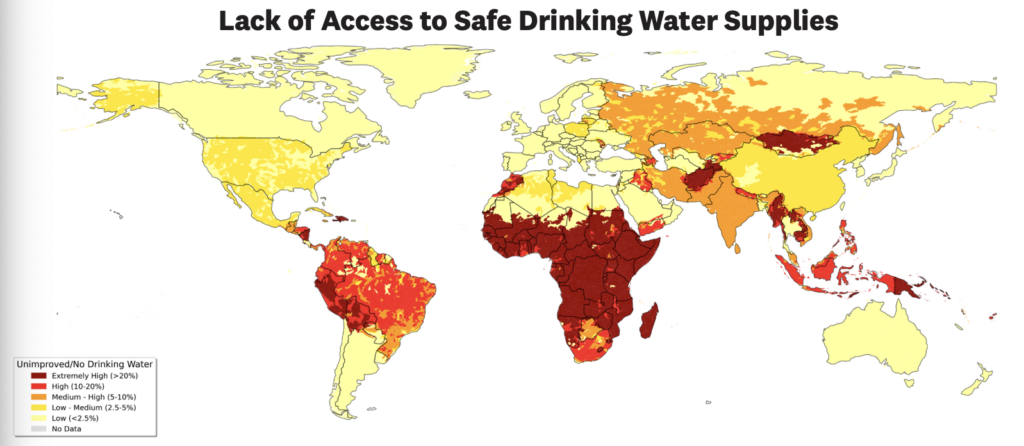
\includegraphics[width=\linewidth]{tcc_images/criseH.png}
    \end{column}
  \end{columns}
  \vfill\hfill{\scriptsize Fontes: WHO, 2023; IDRA, 2026; Imagem: Health Policy Watch, 2024}
  \note{A crise global da água é tanto de quantidade quanto de qualidade. 4 bilhões sofrem com escassez, 1,7 bilhão bebem água contaminada, causando mais de 500 mil mortes por ano. É um problema que demanda soluções urgentes e inovadoras. [~1 min]}
\end{slide}
%========================================================================

\begin{slide}{O Problema no Brasil}
  \begin{columns}[T]
    \begin{column}{.55\linewidth}
      \begin{Item}
        \item 2026: ano desafiador — chuvas abaixo da média; Cantareira $\approx$ 30\% (\textcolor{poliRed}{ANA} — Agência Nacional de Águas)
        \item Nordeste: 4 meses de chuva e 8 meses de seca extrema (ANA)
        \item Dessalinização: em ambientes de escassez, viabiliza desenvolvimento econômico e melhora a qualidade de vida via oferta de água de boa qualidade (estudo \textcolor{poliRed}{CNI}, 2026 \cite{CNI2026})
        \item Maior planta do Brasil (ES): atende demanda de 80 mil pessoas \cite{CNI2026}
        \item 8.500 km de costa $\rightarrow$ enorme potencial para expandir (IBGE)
      \end{Item}
    \end{column}
    \begin{column}{.45\linewidth}
      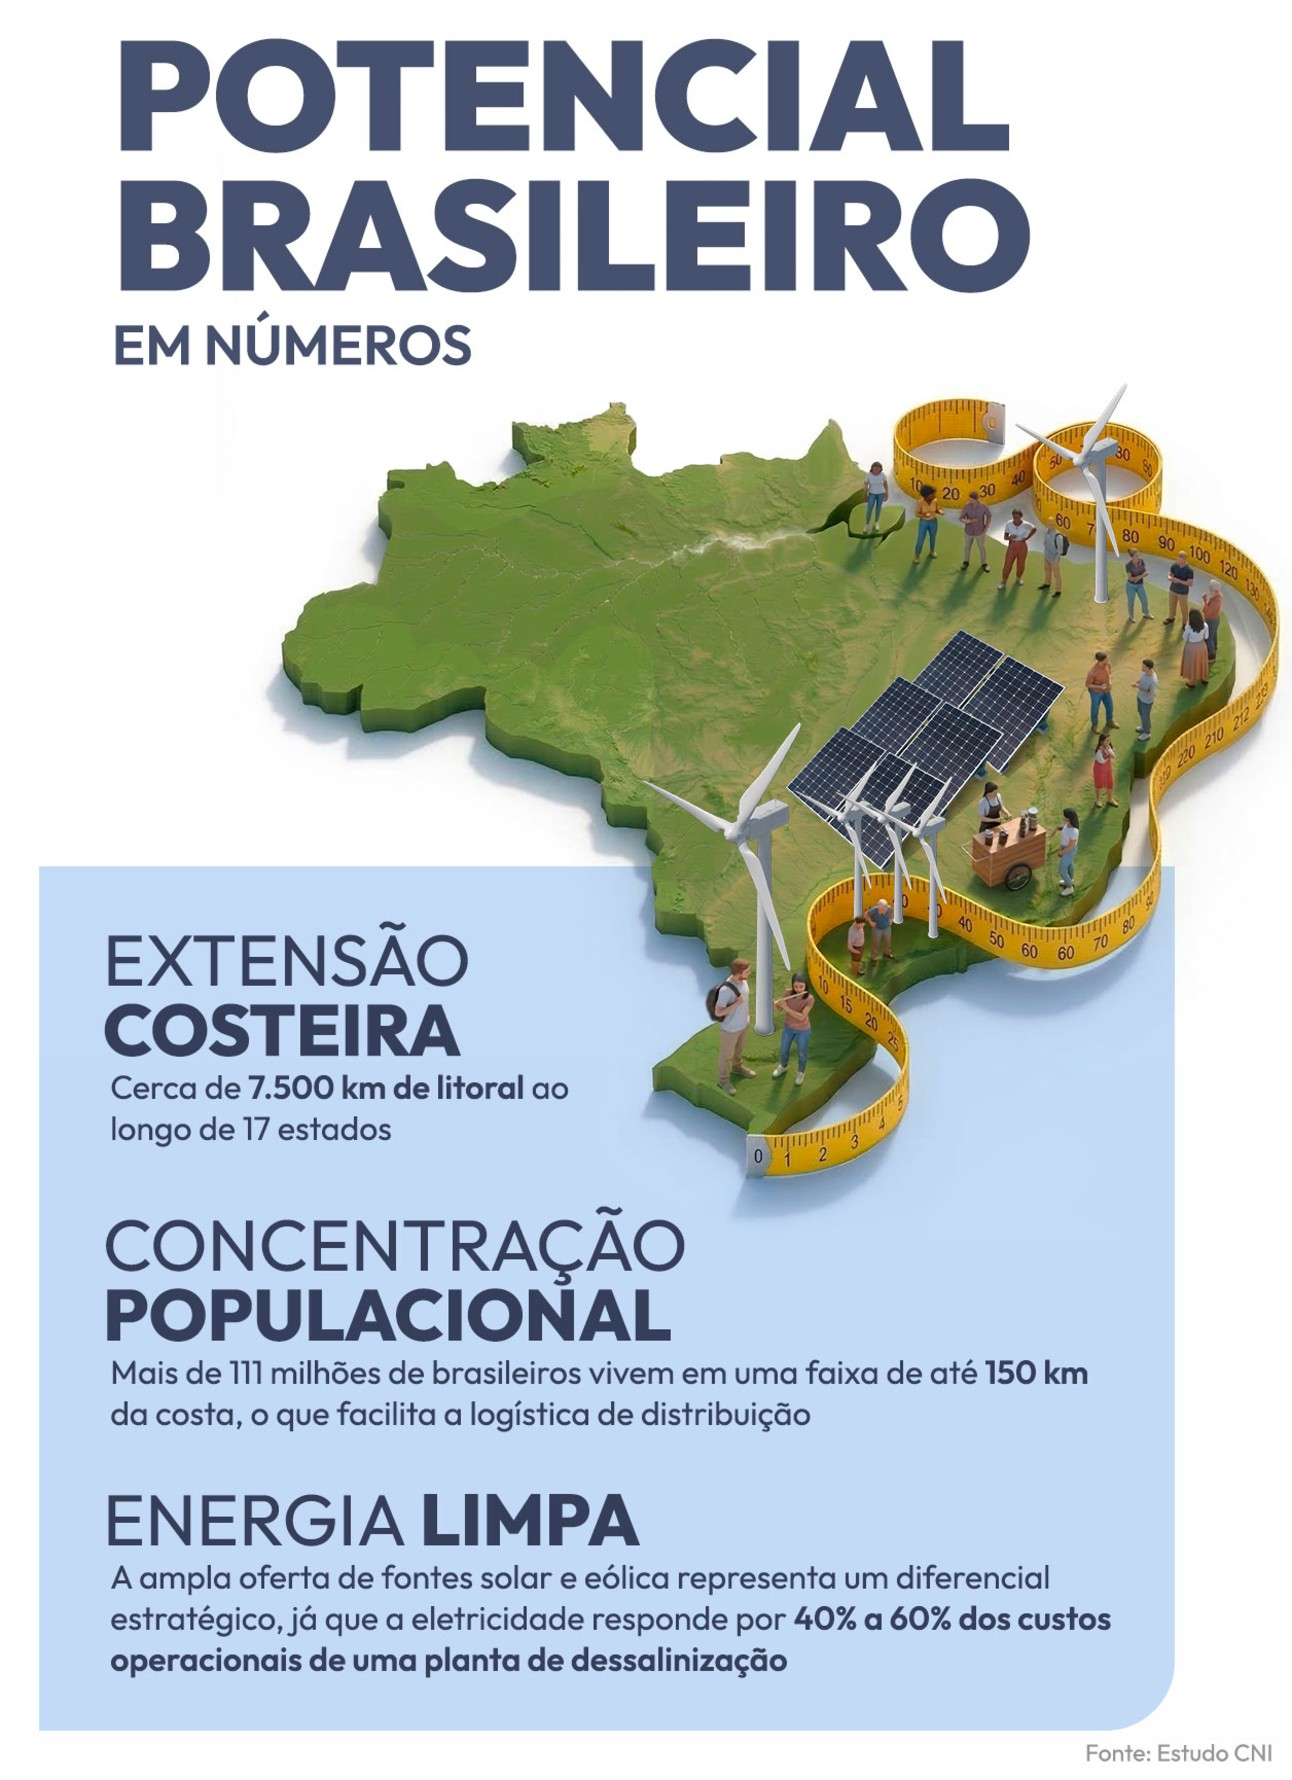
\includegraphics[width=\linewidth]{tcc_images/artebrasillet.jpg}
    \end{column}
  \end{columns}
  \vfill\hfill{\scriptsize Fontes: ANA, 2026; CNI, 2026 \cite{CNI2026}; IBGE; Imagem: CNI, 2026}
   \note{No Brasil, 2026 é desafiante para a gestão de água. O Cantareira está pouco acima de 30\%. No Nordeste, 4 meses de chuva contra 8 de seca extrema. A dessalinização desponta como alternativa estratégica para segurança hídrica segundo estudo da CNI. A maior planta do Brasil, no ES, atende 80 mil pessoas. Com 8.500 km de costa, o potencial de expansão é enorme. [~1 min]}
\end{slide}
%========================================================================

\begin{slide}{O V-AGMD no Contexto da Dessalinização}
  \small
  \begin{columns}
    \begin{column}{.55\linewidth}
      \begin{Item}
        \item \textbf{Dessalinização} divide-se em duas grandes tecnologias:
        \begin{Item}
          \item Processos \textbf{térmicos} (destilação convencional)
          \item Processos de \textbf{membrana} (osmose inversa, MD)
        \end{Item}
        \item \textbf{Destilação por Membrana (MD)}: processo térmico que utiliza uma membrana hidrofóbica para separar o vapor da água da salmoura aquecida
        \item \textcolor{poliRed}{\textbf{V-AGMD}}: configuração que combina \textbf{espaço de ar} (isolamento térmico) com \textbf{vácuo parcial} ($\rightarrow$ menor resistência à transferência de massa do vapor, acelerando o transporte) — foco deste trabalho
      \end{Item}
    \end{column}
    \begin{column}{.4\linewidth}
      \centering
      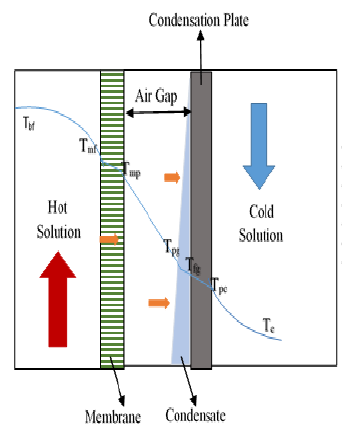
\includegraphics[width=0.85\linewidth]{tcc_images/chap03/Model-of-heat-and-mass-transfer-in-the-AGMD.png}\\[4pt]
      {\tiny Figura: Transporte de calor e massa na MD. Fonte: Zheng (2017)}
    \end{column}
  \end{columns}
  \note{A dessalinização se divide em térmicos e membrana. A MD é um processo térmico que utiliza uma membrana hidrofóbica para separar o vapor d'água. O V-AGMD combina espaço de ar com vácuo: o ar isola termicamente, o vácuo acelera o vapor. [~45s]}
\end{slide}
%========================================================================

\begin{slide}{Ilha de Policogeração Sustentável (LabMEMS/COPPE)}
  \begin{columns}
    \begin{column}{.5\linewidth}
      \begin{Item}
        \item Protótipo pioneiro COPPE/UFRJ (2022): água potável + energia via solar térmica
        \item 5 kW$_e$ ($\approx$ 25 residências) + 8 kW$_t$ recuperáveis em micro-trocadores
        \item Dessalinizador V-AGMD: produz 1.000 L/dia de água destilada ($>$ 100 pessoas/dia)
        \item Foco em comunidades remotas/off-grid (Semiárido, ilhas, O\&G, áreas de desastre)
        \item Potencial complementar a projetos existentes de dessalinização em locais de escassez, como o \textcolor{poliRed}{\textbf{Projeto Água Doce}} (programa federal para o Semiárido nordestino)
      \end{Item}
    \end{column}
    \begin{column}{.5\linewidth}
      \centering
      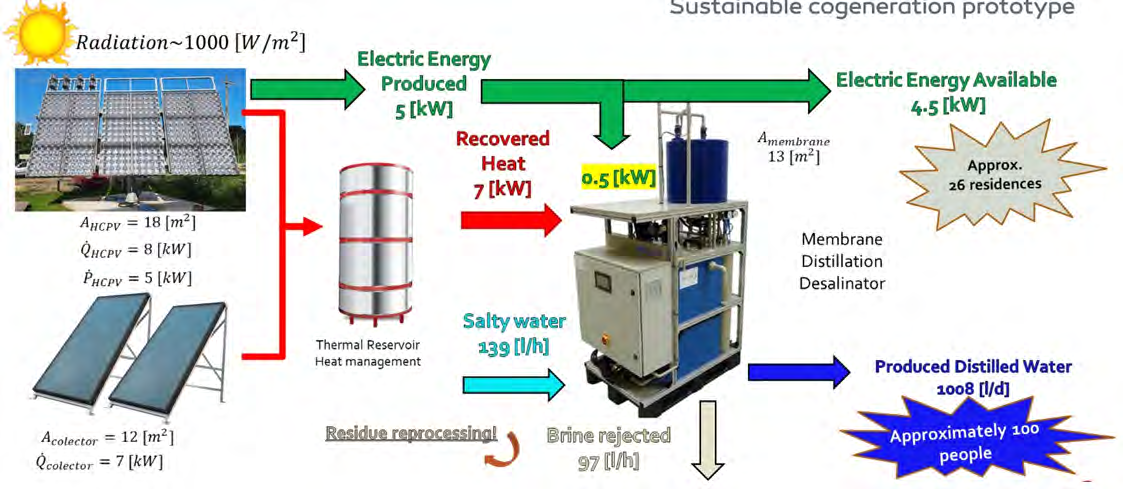
\includegraphics[width=\linewidth]{tcc_images/instalacao_ips.png}
    \end{column}
  \end{columns}
  \vfill\hfill{\scriptsize Fontes: COPPE/UFRJ, 2022; LISBOA et al., 2024; NAVEIRA-COTTA et al. [s.d.]}
  \note{A Ilha de Policogeração Sustentável da COPPE, inaugurada em 2022, é o projeto que abriga este trabalho. É um sistema que integra painéis solares de alta concentração com um dessalinizador V-AGMD, produzindo eletricidade para 25 residências e água para mais de 100 pessoas por dia. O foco são comunidades remotas. Potencial complementar ao Projeto Água Doce. [~1 min]}
\end{slide}
%========================================================================

% Slide da imagem sozinha removido — integrado ao slide anterior
% \begin{slide}{}
%   \vspace*{\fill}
%   \begin{center}
%     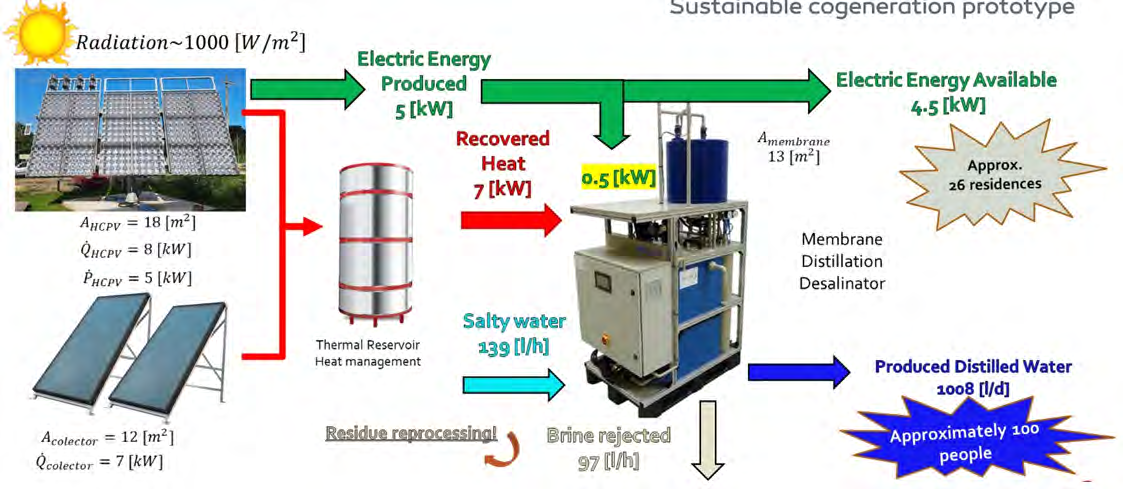
\includegraphics[width=0.9\textwidth, height=0.8\textheight, keepaspectratio]{tcc_images/instalacao_ips.png}
%   \end{center}
%   \vspace*{\fill}
%   \vfill\hfill{\scriptsize Fonte: NAVEIRA-COTTA et al. [s.d.]}
% \end{slide}
%========================================================================

\begin{slide}{Objetivos}
  \footnotesize
  \begin{myTitledBox}[Objetivos]
    \textbf{Objetivo geral:} avaliar e selecionar modelos de regressão supervisionada para predição do desempenho do módulo V-AGMD (fluxo de permeado e temperaturas de saída), combinando aprendizado a partir de dados experimentais (174 pontos, 3 regimes de salinidade) com informação física proveniente de um modelo reduzido 0D já publicado pelo laboratório (LISBOA et al., 2024).
  \end{myTitledBox}
  \note{Objetivo geral: avaliar e selecionar modelos de regressão supervisionada para predição do desempenho do V-AGMD, combinando dados experimentais (174 pontos, 3 regimes) com o modelo físico 0D do laboratório como referência. [~1 min]}
\end{slide}
%========================================================================

\nocite{Abid2020}
\nocite{Lisboa2024}
\endgroup
